\documentclass{article}
\usepackage[utf8]{inputenc}

\usepackage[letterpaper, margin=1in]{geometry}
\usepackage{amsmath}
\usepackage{enumitem}
\usepackage{caption}
\usepackage{subcaption}
\usepackage{graphicx}
\graphicspath{ {figures/} }

\title{Analytical model of pedestrianized and transit priority zones in a rectilinear grid city}
\author{Nicholas Fournier}
\date{February 2020}

\begin{document}


\maketitle

\section{Concept}
Consider an idealized city of dimension $R$ with a rectilinear street network with spacing $d$, as shown in Figure~\ref{fig:gridcity}. Demand can be defined by two types of trip patterns, baseline uniform travel demand across the city and monocentric trips to and from the city center. The cumulative effect is increased congestion in the city center. To make the city center more attractive, ``livable'', and walkable, a square zone of size $\gamma$ in the city center has been pedestrianized, allowing only pedestrians, bicycles, and transits. The pedestrianized zone forces drivers to divert routes around the zone, increasing traffic density and congestion as a result. To mitigate the congestion's impact on mixed-traffic transit (i.e., buses and streetcars/trams), an area of dimension $\tau$ has been designated transit priority, giving transit dedicated lanes. This reduces street capacity for automobiles, but negates the impact of congestion on transit speed.

\begin{figure}[!ht]
     \centering
     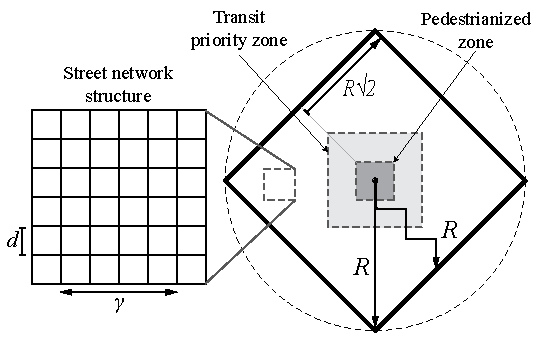
\includegraphics[width=0.5\textwidth]{diagram_pedtransit_grid_city}
     \caption{Rectilinear city with pedestrianized corridor}
     \label{fig:gridcity}
\end{figure}

\noindent The objective is to model the traffic impact on the surrounding street network in order to determine:
\begin{enumerate}[topsep=3pt, itemsep=3pt, partopsep=3pt, parsep=3pt]
    \itshape
    \item what are the optimal pedestrian and transit zone sizes?
    \item what are the impacts on travel time?
    \item what are the resulting shifts in demand?
\end{enumerate}

\section{Demand}
Demand is generated in the city area in units of $\frac{trips}{dist^2}$, and can be simplified into two types: 

\begin{itemize}[topsep=3pt, itemsep=3pt, partopsep=3pt, parsep=3pt]
    \item Uniform baseline travel across the network, $\lambda_b$, and
    \item Monocentric travel demand going to and from the center of the city, $\lambda_c$
\end{itemize}

\noindent The pedestrianized zone will cause some trips to be diverted around the perimeter zone. Trips can be categorized into four distinct types (see Figure~\ref{fig:diverted}:

\begin{enumerate}
	\item routes unaffected by the pedestrianized zone,
	\item routes taking vehicles around the perimeter of the pedestrianized zone to park nearest the destination and the remaining radial distance is traveled on foot,
	\item routes that would have passed through the center travels around the perimeter of the pedestrianized zone vertically, and
	\item routes that would have passed through the center travels around the perimeter of the pedestrianized zone diagonally.
\end{enumerate}

\begin{figure}[!ht]
     \centering
     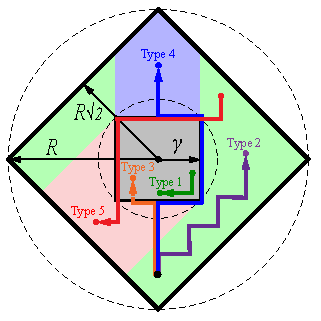
\includegraphics[width=0.3\textwidth]{diagram_diverted_routes}
     \caption{Diverted route types}
     \label{fig:diverted}
\end{figure}

\noindent The flow across the network at a point $r$ distance from the city center is then the summation of this baseline demand and the monocentric demand, calculated as:

\begin{equation}
    q_a(r) = \frac{\lambda_b l}{\delta} + \frac{\lambda_c}{4\delta} \left( \frac{R^2}{r} - r \right)
    \label{eq:flowacross}
\end{equation}

\noindent where $l$ is the average trip link length, $\delta$ is the street density in $\frac{lane \cdot dist}{dist^2}$, calculated as $\delta = \frac{4d}{d^2} = \frac{4}{d}$. The flow around the perimeter road is then calculated as the sum of the flow generated by the four trip types:

\begin{subequations}
\begin{align}
	q_1(\gamma) &= 0 \\
	q_2(\gamma) &= \left[2 \lambda_b \left(R^2 - \gamma^2\right) \times \frac{\gamma^2}{R^2} \times\frac{\gamma}{2}\right] \frac{4d}{8\gamma (R-2)}\\
	q_3(\gamma) &= \left[2 \lambda_b \left(R^2 - \gamma^2\right) \times \frac{\gamma (2R - 3\gamma)}{2R^2} \times  3\gamma\right] \frac{4d}{8\gamma (R-2)}\\
	q_4(\gamma) &= \left[2 \lambda_b \left(R^2 - \gamma^2\right) \times \frac{\gamma (\sqrt{2}R-\gamma)}{R^2} \times  3\gamma\right] \frac{4d}{8\gamma (R-2)}\\
	\notag\text{which can be simplified to:} & \\
	    q_p(\gamma) & = \sum\limits_{i=1}^4 q_i(\gamma) = \frac{\lambda_b d \gamma (6R + 6\sqrt{2}R - 11\gamma)(R^2 - \gamma^2)}{R^2(R-2)}
    \label{eq:perimflow}
\end{align}
\end{subequations}

\noindent The flow across the network at distance $r$ from the center from the function in Equation~\eqref{eq:flowacross} possesses the form shown in Figure~\ref{fig:flowacross}, and flow around the perimeter of the pedestrian zone from the function in Equation~\eqref{eq:perimflow} possesses the form shown in Figure~\ref{fig:perimflow}. As the distance from the city increases, traffic decreases. When traffic near the center exceeds capacity, one might consider simply pedestrianizing the city center out to the point where capacity if first exceeded. However, as the pedestrian zone size increases so does traffic on the perimeter road. 

\begin{figure}[!ht]
     \centering
     \hfill
     \begin{subfigure}[b]{0.45\textwidth}
         \centering
         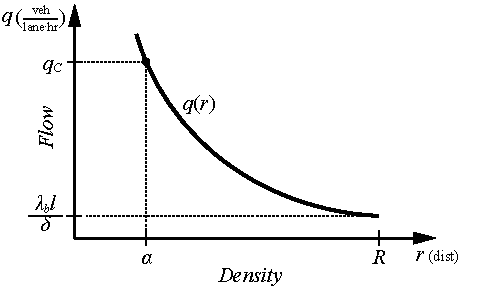
\includegraphics[width=\textwidth]{diagram_flow_across}
         \caption{Trip demand flow at point $r$ distance from center}
         \label{fig:flowacross}
     \end{subfigure}
     \hfill
     \begin{subfigure}[b]{0.45\textwidth}
         \centering
         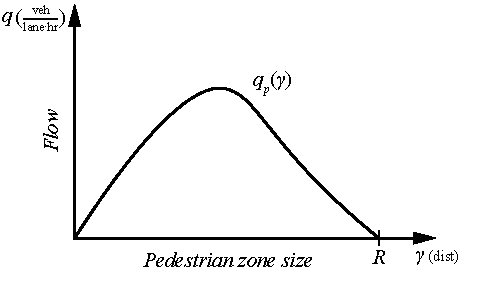
\includegraphics[width=\textwidth]{diagram_flow_perim}
         \caption{Trip demand flow on perimeter of pedestrian zone}
         \label{fig:perimflow}
     \end{subfigure}
     \hfill
     \caption{Macroscopic fundamental diagram and travel time cost function}
\end{figure}



\section{Traffic flow travel time}
Traffic flow through the network is characterized by the macroscopic fundamental diagram (see Figure~\ref{fig:mfd}) as a function of density. A travel time function (see Figure~\ref{fig:traveltime}) then depends upon the state of traffic flow through the network as being either ``uncongested'' (solid line) or ``congested'' (dashed line) in Figures~\ref{fig:mfd} and~\ref{fig:traveltime}.

\begin{figure}[!ht]
     \centering
     \hfill
     \begin{subfigure}[b]{0.45\textwidth}
         \centering
         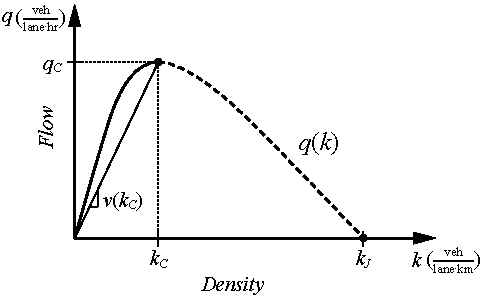
\includegraphics[width=\textwidth]{diagram_mfd}
         \caption{Macroscopic fundamental diagram}
         \label{fig:mfd}
     \end{subfigure}
     \hfill
     \begin{subfigure}[b]{0.45\textwidth}
         \centering
         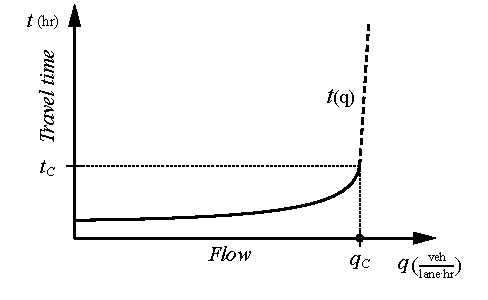
\includegraphics[width=\textwidth]{diagram_traveltime}
        \caption{Travel time cost function}
         \label{fig:traveltime}
     \end{subfigure}
     \hfill
     \caption{Macroscopic fundamental diagram and travel time cost function}
\end{figure}

\noindent A piecewise monotonic cost function for travel time can be defined as:
\begin{subequations}
\begin{align}
    t_D(q) &= l \frac{k(q)}{q} & \text{for}~q < \mu \\
    t_D(q) &= t_c \left(\frac{q}{\mu}\right)  & \text{for}~q \geq \mu
\end{align}
\end{subequations}

\noindent where $t(q)$ is travel time for flow $q$, $k(q)$ is traffic density for flow $q$, $l$ is link length, and $\mu$ is link capacity. Assuming for this case a parabolic function for the uncongested portion of the flow-density relationship, an expression can be written as

\begin{equation}
    q(k) = q_c - (\alpha k - k_c)^2
\end{equation}

\noindent where $k_c$ is the density at capacity, $q_c$ is the flow at capacity, and $\alpha$ is a fitting parameter. In order to determine travel time using density as a function of flow, $k(q)$, it can be solved for using the quadratic formula

\begin{equation}
    k(q) = \frac{k_c - \sqrt{q_c - q}}{\alpha}
\end{equation}


\section{Transit travel time}

Transit travel time is conditional upon whether it operates in a transit priority zone (e.g., dedicated lane or right-of-way) or in mixed-traffic (e.g., city bus). In assuming no other source of delay in a transit priority zone, the travel time of transit is then

\begin{subequations}
\begin{align}
    t_{TP} & = \frac{l}{v_max} + \frac{l}{s}t_s  & \text{with transit priority} \\
    t_{TM}(q) & = l\frac{k(q)}{q} + \frac{l}{s}t_s  & \text{without transit priority when}~q \geq \mu\\
    t_{TM}(q) & = t_c \left(\frac{q}{\mu}\right) + \frac{l}{s}t_s & \text{without transit priority when}~q \geq \mu
\end{align}
\end{subequations}

\noindent where $v_max$ is the maximum cruising speed of transit unimpeded by traffic, $s$ is stop spacing, and $t_s$ is stop time. The stop time is essentially the lost time inclusive of acceleration, deceleration and dwell time.

The travel time of transit in mixed-traffic will then always higher than driving an automobile, eventually converging as traffic conditions reach capacity. Transit priority provides a constant travel time which will be initially slower than driving in uncongested traffic conditions, but will eventually reach a traffic flow point $q^*_T$, where the travel time of transit with priority exceeds driving (see Figure~\ref{fig:transittraveltime}). 

\begin{figure}[!ht]
     \centering
     \hfill
     \begin{subfigure}[b]{0.45\textwidth}
         \centering
         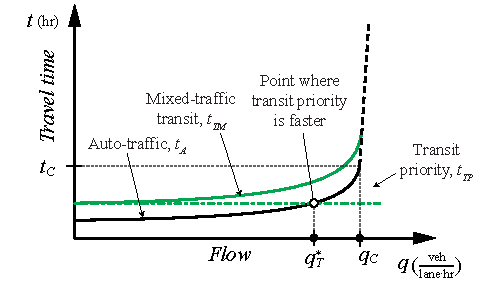
\includegraphics[width=\textwidth]{diagram_transit_traveltime}
        \caption{Transit travel time}
         \label{fig:transittraveltime}
     \end{subfigure}
     \hfill
     \begin{subfigure}[b]{0.45\textwidth}
         \centering
         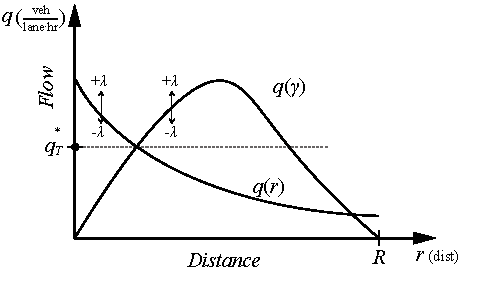
\includegraphics[width=\textwidth]{diagram_flow_combo}
         \caption{Optimal pedestrian and transit priority zone size}
         \label{fig:flowcombo}
     \end{subfigure}
     \hfill
     \caption{Transit travel time and optimal zone sizing}
\end{figure}

The critical transit traffic flow point $q^*_T$ could be used in combination with network flow at distance $r$ in Equation~\eqref{eq:flowacross} to determine the optimal transit priority zone, $\tau$. However, if transit draw trips away from driving, $\pm \lambda_D$, it would thus reduce congestion and improve driving travel time, resulting in more driving trips. Assuming transit provides a reliable alternative to driving, some demand equilibrium exists where the travel time cost of driving matches transit.

An appropriate pedestrian zone size can exist anywhere in the range $q_a(\gamma) < q_c > q_p(\gamma)$ where the pedestrian zone is:
\begin{enumerate}[label=(\alph*)]
    \item large enough to prevent traffic flow across the network from exceeding capacity $q_a(\gamma) < q_c$, and 
    \item small enough to prevent perimeter traffic flow from exceeding capacity $q_p(\gamma) < q_c$. 
\end{enumerate}

While the intersection point of the two functions may be used as an optimal compromise ensuring both conditions are satisfied with the least possible traffic flow. Solving for the intersection point becomes a quintic function (polynomial to the $5^{th}$ power) that is not easily solvable analytically. However, given that the pedestrian zone size must exist between $0 \leq \gamma \leq R$, an exact deterministic solution for optimal pedestrian zone dimension $\gamma^*$, is found when the function is zero (i.e., $q_a(\gamma) = q_p(\gamma)$:

\begin{equation}\small
\gamma^* \Leftarrow \text{min} f(\tau) = 0 = \frac{11}{R^2} \gamma^5 - \frac{6(1+\sqrt{2})}{R}\gamma^4 - 11\gamma^3 + \frac{24\delta\lambda_b d R(1+\sqrt{2}) + \lambda_{c}(R-2)}{4\delta\lambda_{b}d}\gamma^{2} - \frac{R(R-2)}{\delta d}\gamma - \frac{\lambda_{c}(R-2)R^{2}}{4\delta\lambda_{b}d}
\end{equation}


\section{Mode choice}

The mode choice can be modeled as the probability of choosing to drive $P_D$ or transit $P_T$, using a simple two-alternative logit model with (dis-)utility as the choice travel cost:

\begin{subequations}
    \label{eq:choiceprob}
    \begin{align}
        P_D & = \frac{1}{1+e^{-\beta (t_D-t_T)}}\\
        P_T & = 1 - P_D
    \end{align}
\end{subequations}

\noindent where $t_A$ and $t_T$ are the travel times associated with automobile and transit, respectively; and $\beta$ is the a estimated scaling parameter. The probability in Equation~\eqref{eq:choiceprob} can be used to find the proportion of trips made by driving.


\section{...}

Since the logit only requires a differential we just need $\Delta t = t_D - t_T$:

\begin{equation}
    \Delta t(q) = l \frac{k(q)}{q} - \left[
    \frac{\tau}{R} \left( \frac{l}{v_T} + \frac{l}{s}t_s \right) + \frac{R-\tau}{R} \left( l\frac{k(q)}{q} + \frac{l}{s}t_s \right) \right]
\end{equation}

\noindent Since $q^*_T$ is a global constant regardless of demand, we can get $\tau$ by setting $q_a(\tau)=q^*_T$. But $q_a$ depends on demand, which depends on probability, which depends on travel time.

\begin{align}
    q_a(\tau, \Delta t(q)) & = P_D(\Delta t(q)) \times \left[ \frac{\lambda_b l}{\delta} + \frac{\lambda_c}{4\delta} \left( \frac{R^2}{\tau} - \tau \right) \right] \\
    q_a(\tau, \Delta t(q)) & = q^*_T
\end{align}

\noindent Now there is some sort of dynamic equilibrium with flow and demand where travel time depends on flow and flow depends on travel time. 

The pedestrian zone size somewhat less critical since it can exist in a range. However, lets set boundary as the perimeter flow.

\begin{equation}
        q_p(\gamma, \Delta t(q)) = P_D(\Delta t(q)) \times \frac{\lambda_b d \gamma (R^2 - \gamma^2) (3R + 3\sqrt{2}R - 7\gamma)}{R^2(R-2)} < q_c
\end{equation}


\end{document}
